
\documentclass[11pt,letterpaper]{article}\usepackage[]{graphicx}\usepackage[]{color}
%% maxwidth is the original width if it is less than linewidth
%% otherwise use linewidth (to make sure the graphics do not exceed the margin)
\makeatletter
\def\maxwidth{ %
  \ifdim\Gin@nat@width>\linewidth
    \linewidth
  \else
    \Gin@nat@width
  \fi
}
\makeatother

\definecolor{fgcolor}{rgb}{0.345, 0.345, 0.345}
\newcommand{\hlnum}[1]{\textcolor[rgb]{0.686,0.059,0.569}{#1}}%
\newcommand{\hlstr}[1]{\textcolor[rgb]{0.192,0.494,0.8}{#1}}%
\newcommand{\hlcom}[1]{\textcolor[rgb]{0.678,0.584,0.686}{\textit{#1}}}%
\newcommand{\hlopt}[1]{\textcolor[rgb]{0,0,0}{#1}}%
\newcommand{\hlstd}[1]{\textcolor[rgb]{0.345,0.345,0.345}{#1}}%
\newcommand{\hlkwa}[1]{\textcolor[rgb]{0.161,0.373,0.58}{\textbf{#1}}}%
\newcommand{\hlkwb}[1]{\textcolor[rgb]{0.69,0.353,0.396}{#1}}%
\newcommand{\hlkwc}[1]{\textcolor[rgb]{0.333,0.667,0.333}{#1}}%
\newcommand{\hlkwd}[1]{\textcolor[rgb]{0.737,0.353,0.396}{\textbf{#1}}}%

\usepackage{framed}
\makeatletter
\newenvironment{kframe}{%
 \def\at@end@of@kframe{}%
 \ifinner\ifhmode%
  \def\at@end@of@kframe{\end{minipage}}%
  \begin{minipage}{\columnwidth}%
 \fi\fi%
 \def\FrameCommand##1{\hskip\@totalleftmargin \hskip-\fboxsep
 \colorbox{shadecolor}{##1}\hskip-\fboxsep
     % There is no \\@totalrightmargin, so:
     \hskip-\linewidth \hskip-\@totalleftmargin \hskip\columnwidth}%
 \MakeFramed {\advance\hsize-\width
   \@totalleftmargin\z@ \linewidth\hsize
   \@setminipage}}%
 {\par\unskip\endMakeFramed%
 \at@end@of@kframe}
\makeatother

\definecolor{shadecolor}{rgb}{.97, .97, .97}
\definecolor{messagecolor}{rgb}{0, 0, 0}
\definecolor{warningcolor}{rgb}{1, 0, 1}
\definecolor{errorcolor}{rgb}{1, 0, 0}
\newenvironment{knitrout}{}{} % an empty environment to be redefined in TeX

\usepackage{alltt}
\usepackage[utf8]{inputenc}
\usepackage{authblk}
\usepackage{multicol}
\usepackage{graphicx}
\usepackage{threeparttable}
\usepackage[unicode=true]{hyperref}
\hypersetup{breaklinks=true,
            bookmarks=true,
            colorlinks=true,
            citecolor=blue,
            urlcolor=blue,
            linkcolor=magenta,
            pdfborder={0 0 0}}
\urlstyle{same}
\setlength{\columnsep}{1cm}
\usepackage[left=1.5cm,right=1.5cm,top=1.5cm,bottom=1.5cm]{geometry}
\title{\textbf{Clinicopathologic and Outcome Features of Superficial High-Grade and Deep Low-Grade Squamous Cell Carcinomas of the Penis}}
\author{Alcides Chaux, M.D.\textsuperscript{1,2}}
\date{}
\IfFileExists{upquote.sty}{\usepackage{upquote}}{}
\begin{document}

\maketitle

\begin{abstract}

\textbf{Objetives:} To report the clinicopathologic and outcome features of superficial high-grade and deep low-grade penile squamous cell carcinomas.

\textbf{Methods:} From a retrospectively-collected series of patients with penile cancer we identified 41 cases corresponding to 12 superficial high-grade tumors and 29 deep low-grade tumors. As outcomes we evaluated inguinal lymph node status, presence of tumor relapse, final nodal status, and cancer-specific death. Follow-up ranged from 0.8 to 386.7 months (mean, 152.5 months; median, 157.3 months).

\textbf{Results:} Clinicopathologic features were similar between superficial high-grade and deep low-grade tumors, except for a tendendy (Fisher's exact $P=0.057$) of the former to include tumors with a verruciform pattern of growth. A significantly higher proportion of inguinal lymph node metastasis was found in superficial high-grade tumors compared to deep low-grade tumors [4/5 (80\%) vs. 1/5 (20\%) respectively, Fisher's exact $P=0.02$]. No significant differences were found regarding tumor relapse (Fisher's exact $P=0.52$), final nodal status (Mantel-Cox's $P=0.42$), or cancer-related death (Mantel-Cox's $P=0.52$).

\textbf{Conclusions:} Our findings suggest that patients with superficial high-grade tumors may be treated differently from patients with deep low-grade tumors, at least to control short-term local disease. Prophylactic inguinal lymphadenectomuy might be indicated in cases of superficial tumors with high-grade histology while in deeply invasive low-grade penile carcinomas a more conservative approach may be considered.\\

\textbf{Keywords:} penile cancer; squamous cell carcinoma; histological grade; prognostic factors; outcome; anatomical level.

\end{abstract}

\let\thefootnote\relax\footnote{
\\ \textbf{Author Affiliation:} \textsuperscript{1}Department of Scientific Research, Norte University, Paraguay; \textsuperscript{2}Centro para el Desarrollo de la Investigación Científica, Asunción, Paraguay.
}
\let\thefootnote\relax\footnote{
\\ \textbf{Corresponding Author:} Alcides Chaux, M.D. Department of Scientific Research, Norte University, Gral. Santos e/ 25 de Mayo, Asunción, Paraguay. Office: +595 (021) 203-108, ext. 142. Email: \href{mailto:alcideschaux@uninorte.edu.py}{alcideschaux@uninorte.edu.py}
}

\begin{multicols}{2}

\section*{Introduction}
Pathologic features of the primary tumor affecting outcome of patients with penile cancer are multiple and include histological grade \cite{Chaux2009,Chaux2009b,Velazquez2008}, percentage of anaplastic cells \cite{Slaton2001}, anatomical level of infiltration \cite{Chaux2009}, depth of invasion \cite{Dai2006,Emerson2001}, tumor stage \cite{Slaton2001,Dai2006,Guimaraes2006}, presence of vascular \cite{Slaton2001,Emerson2001,Guimaraes2006,Ficarra2005} and perineural \cite{Chaux2009,Velazquez2008} invasion, histological subtype \cite{Dai2006,Guimaraes2009} and tumor front of invasion \cite{Guimaraes2006}. Risk groups systems combine histological grade with tumor extension to estimate the likelihood of inguinal nodal involvement \cite{Solsona2001,Solsona2004,Hungerhuber2006,Ornellas2008}. The combination of histological grade, anatomical level of invasion and presence of perineural invasion was found to be strongly related to nodal involvement and cancer-specific survival \cite{Chaux2009}. Similarly to other malignancies, in penile cancer depth of tumor invasion and histologic grade are frequently and significantly associated \cite{Guimaraes2009}. However, we have occasionally found superficial tumors depicting a high histological grade and deeply infiltrating malignant neoplasms showing a low-grade histology. The purpose of this study was to evaluate the clinicopathologic and outcome features of patients with such ``paradoxical'' tumors.

\section*{Material \& Method}

\subsection*{Cohort of Patients}
Patients were selected from a previously published series of 333 patients with invasive penile squamous cell carcinoma \cite{Guimaraes2009}. This dataset is publicly available at \url{http://dx.doi.org/10.6084/m9.figshare.1290997}.

\subsection*{Classification of Cases}
The dataset was searched for tumors fulfilling the following criteria:

\begin{description}
        \item[Superficial High-Grade Tumors:] Grade 3 tumors invading lamina propria or superficial corpus spongiosum (tumor thickness $\leq$ 5 mm).
        \item[Deep Low-Grade Tumors:] Grade 1 tumors invading deep corpus spongiosum (tumor thickness $\geq$ 10 mm) or corpus cavernosum, including tunica albuginea.
\end{description}

The cutoff points of 5 mm and 10 mm were selected based on previous studies \cite{Velazquez2008}. Tumors not fulfilling these criteria were excluded from the dataset. Patients who were lost at follow-up were also excluded. The final count of selected cases for data analysis was 41, which included 12 (29\%) superficial high-grade tumors and 29 (71\%) deep low-grade tumors.

\subsection*{Follow-Up}
Patients were followed-up from 0.8 to 386.7 months (mean, 152.5 months; median, 157.3 months). Two endpoints were evaluated during follow-up:
\begin{enumerate}
        \item \textbf{Tumor relapse:} tumor relapse included the development of local relapse (i.e., tumor on stump), regional relapse (i.e., metastases in regional lymph nodes), or systemic relapse (i.e., metastases in systemic lymph nodes, visceral metastases) during follow-up.
        \item \textbf{Outcome:} the possible categories of outcome included alive without disease, alive with disease, died of other causes, and died of cancer.
\end{enumerate}

\subsection*{Final Lymph Nodes Status}
The final status of inguinal lymph nodes was established as follows: 
\begin{enumerate}
        \item \textbf{Positive status:} the final nodal status was considered positive if pathologically-proven nodal metastases were observed (in those cases with inguinal lymphadenectomy), if regional relapse appeared during follow-up, or if the outcome was unfavorable (i.e., alive with disease or death by cancer).
        \item \textbf{Negative status:} the final nodal status was considered negative if nodal metastases were not observed (in those cases with inguinal lymphadenectomy), if no tumor relapse (beyond local relapse) appeared during follow-up, or if the outcome was favorable (i.e., alive without disease or death by other causes).
\end{enumerate}

\subsection*{Statistical analyses}
Bivariate analyses were carried out using the Fisher's exact test for contingency tables and the Kruskal-Wallis rank sum test for grouped numerical variables. Survival curves were generated using the Kaplan-Meier method and compared with the log-rank (Mantel-Cox) test. Unconditional logistic regression models were built to estimate odds ratios and 95\% confidence intervals. In all cases a 2-tailed $P\textless 0.05$ was required for statistical significance. Data were analyzed and plots were generated using R version 3.1.2 ``Pumpkin Helmet'' \cite{RCoreTeam}. The dataset and R scripts used for data analysis, as well as additional results (including the full analysis of the dataset), are freely available at \url{https://github.com/alcideschaux/Penis-Paradoxical}.

\section*{Results}
Table \ref{Table_Distribution} compares the clinicopathologic and outcome features of patiens with superficial high-grade and deep low-grade tumors. None of the clinicopathologic features were significantly associated with the type of tumor, althought deep low-grade tumors tended to exhibit a verruciform pattern of growth. Of the outcome features, only the presence of inguinal lymph node metastasis was significantly different between superficial high-grade and deep low-grade tumors, with a higher proportion of metastasis in the latter [4/5 (80\%) cases] compared to the former [1/5 (20\%) cases].

% Beginning of TABLE %
\begin{table*}
\centering
\caption{Clinicopathologic and Outcome Features of Superficial High-Grade and Deep Low-Grade Tumors}
\label{Table_Distribution}
\begin{tabular}{lccl}
\hline
~ & \textbf{Superficial High-Grade} & \textbf{Deep Low-Grade} & \textbf{P value} \\
\hline
No. cases (\%)  & 12 (29\%)
                & 29 (71\%)
                & ~ \\

\textbf{Clinical Features} & ~ & ~ & ~ \\
\hspace{2ex} Patients's age in years, median (IQR)
        & 52.5 (12.5)
        & 56 (19)
        & 0.11 \\
\hspace{2ex} Tumor size in cm, median (IQR)
        & 4.5 (4.125)
        & 5 (2.125)
        & 0.95 \\
\hspace{2ex} Anatomical location (\%) & ~ & ~ & 0.89 \\
\hspace{4ex} Glans alone
        & 7/26 (27\%)
        & 19/26 (73\%)
        & ~ \\
\hspace{4ex} Glans + Coronal sulcus
        & 2/6 (33\%)
        & 4/6 (67\%)
        & ~ \\
\hspace{4ex} Glans + Coronal sulcus + Forsekin
        & 3/9 (33\%)
        & 6/9 (67\%)
        & ~ \\

\textbf{Pathologic Features} & ~ & ~ & ~ \\
\hspace{2ex} Histologic subtype (\%) & ~ & ~ & 0.057 \\
\hspace{4ex} Usual SCC
        & 11/24 (46\%)
        & 13/24 (54\%)
        & ~ \\
\hspace{4ex} Verrucous carcinoma
        & 0/7 (0\%)
        & 7/7 (100\%)
        & ~ \\
\hspace{4ex} Papillary carcinoma
        & 0/3 (0\%)
        & 3/3 (100\%)
        & ~ \\
\hspace{4ex} Warty carcinoma
        & 1/3 (33\%)
        & 2/3 (67\%)
        & ~ \\
\hspace{4ex} Mixed carcinoma
        & 0/4 (0\%)
        & 4/4 (100\%)
        & ~ \\

\hspace{2ex} Urethral invasion (\%) & ~ & ~ & 0.7 \\
\hspace{4ex} Positive
        & 3/15 (20\%)
        & 12/15 (80\%)
        & ~ \\
\hspace{4ex} Negative
        & 6/19 (32\%)
        & 13/19 (68\%)
        & ~ \\

\hspace{2ex} Perineural invasion (\%) & ~ & ~ & 1 \\
\hspace{4ex} Positive
        & 2/6 (33\%)
        & 4/6 (67\%)
        & ~ \\
\hspace{4ex} Negative
        & 10/34 (29\%)
        & 24/34 (71\%)
        & ~ \\

\hspace{2ex} Vascular invasion (\%) & ~ & ~ & 0.57 \\
\hspace{4ex} Positive
        & 2/4 (50\%)
        & 2/4 (50\%)
        & ~ \\
\hspace{4ex} Negative
        & 10/36 (28\%)
        & 26/36 (72\%)
        & ~ \\

\textbf{Outcome Features} & ~ & ~ & ~ \\
\hspace{2ex} Inguinal lymph node metastasis (\%) & ~ & ~ & 0.02 \\
\hspace{4ex} Positive
        & 4/5 (80\%)
        & 1/5 (20\%)
        & ~ \\
\hspace{4ex} Negative
        & 8/36 (22\%)
        & 28/36 (78\%)
        & ~ \\

\hspace{2ex} Tumor relapse (\%) & ~ & ~ & 0.52 \\
\hspace{4ex} Local, regional or systemic relapse
        & 1/2 (50\%)
        & 1/2 (50\%)
        & ~ \\
\hspace{4ex} No tumor relapse
        & 11/38 (29\%)
        & 27/38 (71\%)
        & ~ \\

\hspace{2ex} Final nodal status (\%) & ~ & ~ & 0.2 \\
\hspace{4ex} Positive
        & 4/8 (50\%)
        & 4/8 (50\%)
        & ~ \\
\hspace{4ex} Negative
        & 8/33 (24\%)
        & 25/33 (76\%)
        & ~ \\

\hspace{2ex} Death by disseminated cancer (\%) & ~ & ~ & 1 \\
\hspace{4ex} Positive
        & 0/1 (0\%)
        & 1/1 (100\%)
        & ~ \\
\hspace{4ex} Negative
        & 12/40 (30\%)
        & 28/40 (70\%)
        & ~ \\
\hline
\end{tabular}
\end{table*}

% End of TABLE %


Table \ref{Table_OR} shows the results of the logistic regression analysis for predicting outcomes based on the type of tumor. Patients with superficial high-grade tumors had an significantly increased risk for inguinal lymph node metastasis compared to patients with deep low-grade tumors. Risks were not significantly different for tumor relapse or final nodal status. Risk for cancer-related death was not evaluable due to the small number of events.

Figure \ref{Fig_Survival} shows the survival curves for final nodal status and cancer-related death by type of tumor. As seen, no significant differences were observed between patients with superficial high-grade and deep low-grade tumors in regards to the aforementioned outcomes.

\section*{Discussion}

% Beginning of TABLE %
\begin{table*}
\centering
\caption{Odds Ratios for Predicting Outcomes in Superficial High-Grade vs. Deep Low-Grade Tumors}
\label{Table_OR}
\begin{tabular}{lccl}
\hline
\textbf{Outcome} & \textbf{Odds Ratio} & \textbf{95\% Confidence Intervals} & \textbf{P value} \\
\hline
Inguinal lymph node metastasis
        & 14
        &   1.8, 295.7
        & 0.026 \\
Tumor relapse
        & 2.5
        &  0.09, 65.89
        & 0.54 \\
Final nodal status
        & 3.1
        &  0.61, 16.27
        & 0.16 \\
Death by disseminated cancer
        & 3.3e-08
        &  NA, Inf
        & 1 \\
\hline
\end{tabular}
\begin{tablenotes}
\small
\item NA, not available; Inf, infinite.
\end{tablenotes}
\end{table*}
% End of TABLE

In this study we analyzed the clinicopathologic and outcome features of patients with superficial high-grade and deep low-grade squamous cell carcinomas of the penis. We found no significant differences in the clinicopathologic features, except for some tendency of low-grade tumors to exhibit a verruciform pattern of growth. Regarding outcome, superficial high-grade tumors showed a higher proportion of inguinal lymph node metastasis compare to deep low-grade tumors, suggesting that histologic grade is more influential on prognosis than depth of invasion in this particular setting. Nevertheless, the type of tumor had limited usefulness in predicting nodal disease (i.e., final nodal status) or cancer-related death, indicating that other factors should be taken into account for prediciting long-term outcome. Our results suggest that patients with superficial high-grade tumors may benefit from a more aggresive approach (v.g., prophylactic inguinal lymphadenectomy), in spite of their lower pT stage. Conversely, patients with deep low-grade tumors could be suitable candidates for an active surveillance program instead of a more aggresive approach, despite their higher pT stage.

Our results are in agreement with a previous study evaluating penile tumors invading 5 to 10 mm, in which histologic grade had more influence on prognosis than depth of tumor invasion \cite{Velazquez2008}. Given its importance and clinical implications histological grading should be carried out using uniform and comparable criteria, moreover considering that a significant interobsarver variability has been reported for histologic grading in penile carcinomas \cite{Naumann2009}. For patients included in this study, histologic grading was carried out using strict (and previously validated) morphologic criteria \cite{Chaux2009b}. This approach may reduce interobserver variability, althought further studies are required to evaluate the external validity and reproducibility of such criteria.

In addition, to consider only the T stage of the penile tumor to define the type and extension of primary treatment could be misleading. Some tumor variants, such as basaloid, sarcomatoid and high-grade usual carcinomas are intrinsically aggressive, regardless of the anatomical level of infiltration\cite{Chaux2009a,Velazquez2005,Guimaraes2009}. Other tumor variants, such as carcinoma cuniculatum, could invade deep erectile tissues and nevertheless be associated with good prognosis \cite{Barreto2007}. Moreover, the current TNM system for penile cancer considers invasion of corpus spongiosum or corpus cavernosum as a single pT2 category \cite{Hakenberg2015}. Previous studies have found that the metastatic rate of tumors invading corpus cavernosum is higher than those tumors limited to corpus spongiosum \cite{Chaux2009}. Furthermore, splitting the pT2 stage in 2 categories depending on invasion of corpus spongiosum vs. corpus cavernosum has proven useful in increasing the accuracy of the TNM sytem for predicting outcome \cite{Leijte2008}. It does not seem advisable to rely solely on the pT stage to plan optimal therapeutic management. An anatomical level-based approach, combined or not with measurement of tumor thickness, has been evaluated and found useful \cite{Chaux2009,Velazquez2008}. Information on histologic grade should be included in pathologic reports and anatomical level of infiltration weighted with this grading in order to plan optimal management of patients with penile cancer.

As mentioned before, tumors with a verruciform pattern of growth predominated in the deep low-grade category. Tumors with verrucous features includs verrucous carcinoma, papillary, and warty carcinomas \cite{Chaux2010b,Chaux2012}. Verrucous carcinomas were characterized by prominent acanthosis, inconspicuous fibrovascular cores, hyperkeratosis and a broad pushing base. It is noteworthy that, although verrucous carcinomas are considered as non-invasive tumors in the latest TNM classification system \cite{Hakenberg2015}, they can affect deep erectile tissues, as shown in this study. Low-grade warty and papillary carcinomas were very similar in their pattern of growth but papillae were more irregular and architecturally complex in papillary carcinomas and koilocytosis were easily found in warty carcinomas. The superficial high-grade category included high-grade usual and warty carcinomas. High-grade usual SCC was characterized by nuclear pleomorphism, irregular nuclear membrane, coarse chromatin, prominent nucleoli and high mitotic rate. The other subtype found in the superficial high-grade category was high-grade warty carcinoma, a tumor depicting all the typical aforementioned features of a warty carcinoma (papillae with prominent fibrovascular cores, conspicuous koilocytosis, and jagged tumor base) but showing areas of anaplastic cells, usually at the tumor front of invasion.

\begin{figure*}
\centering
\begin{knitrout}
\definecolor{shadecolor}{rgb}{0.969, 0.969, 0.969}\color{fgcolor}
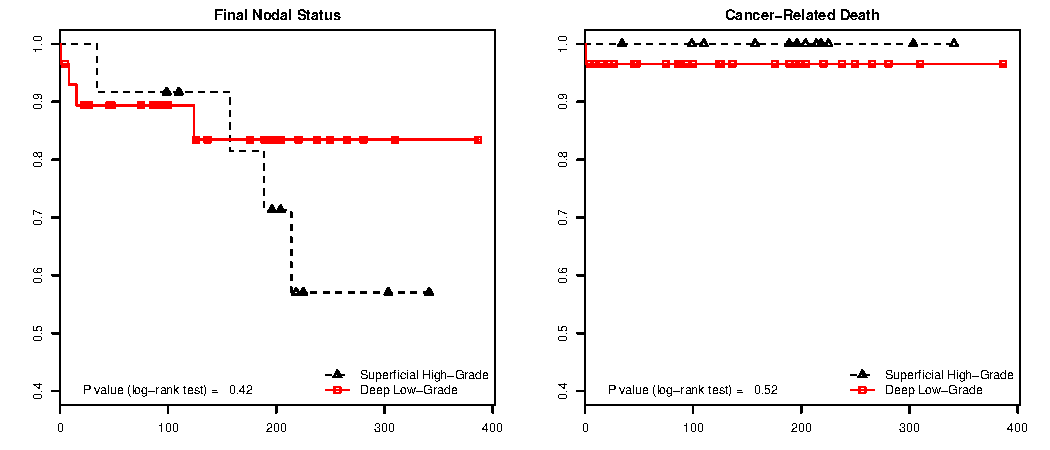
\includegraphics[width=\maxwidth]{figure/Survival-1} 

\end{knitrout}
        \caption{Survival curves for final nodal status and cancer-related death by type of tumor. No significant differences were found in the survival curves. Follow-up in months is depicted in the x-axes, while the y-axes depict survival functions.}
        \label{Fig_Survival}
\end{figure*}

Some limitations must be acknowledged. Our study is based on a retrospectively-collected series of cases. As such, clinical features were gathered form clinical reports and pathologic features were evaluated only on available microscopic slides. This might have had an impact in the quality of the data that is hard to estimate. Clearly, similar studies (preferibly with prospectively-collected data) on large datasets of patients with penile cancer are required to determine if the differences and similarities we found are constant features of these type of tumors. Notwithstanding these limitations, our study suggests that patients with superficial high-grade and deep low-grade tumors might benefit from a different therapeutic management than the approach used in more usual clinical settings.

In conclusion, whereas in the majority of penile carcinomas higher grade and deeper tumor invasion are significantly associated, there are cases in which a high-grade tumor may invade only superficially and low-grade tumors can affect deep erectile tissues. Tumors with such features were identified in about 8\% of all cases in a large dataset of patients with penile squamous cell carcinomas. We found that superficial high-grade tumors had a significantly higher proportion of inguinal lymph node metastasis compared to deep low-grade tumors. Our findings might indicate that patients with superficial high-grade tumors should be treated differently from patients with deep low-grade tumors, at least to control short-term local disease. On this regard, prophylactic inguinal lymphadenectomuy might be indicated in cases of superficial tumors with high-grade histology while in deeply invasive low-grade penile carcinomas a more conservative approach may be considered.

\section*{Conflict of Interest}
The author declare no conflict of interest.

\section*{Financial Disclosure}
Dr. Alcides Chaux was partially supported by an award granted by the National Council of Science and Technology (CONACYT) dependent of the Presidency of the Republic of Paraguay, as a Level 2 Active Researcher of the National Incentive Program for Researchers (PRONII).

\bibliographystyle{unsrt}
\bibliography{References}

\end{multicols}

\end{document}
